\documentclass[12pt, letterpaper]{article}
\usepackage[utf8]{inputenc}
\usepackage{graphicx}
\usepackage{fullpage}
\usepackage{setspace}
\usepackage{biblatex}
\usepackage{mathtools}
\usepackage{appendix}
\usepackage[version=4]{mhchem}
\usepackage[export]{adjustbox}
\usepackage{pdflscape}
\usepackage{amsmath}
\usepackage{units}
\usepackage{booktabs}
\usepackage[pdftex,bookmarks=true,bookmarksnumbered=true,colorlinks=true,linkcolor=blue,urlcolor=red,citecolor=green,filecolor=magenta]{hyperref}
\graphicspath{{Images/}}
\addbibresource{main.bib}
\doublespacing

\title{Modeling an MEA Absorption Column with the Sequential Shooting Method}
\author{Tanner Polley}
\date{\today}

\begin{document}
    \maketitle
    \begin{abstract}
        Sentence about the importance of carbon capture and developing its technology.
        Sentence about Post Combustion Carbon Capture.
        Sentence about amine-based absorption.
        Sentence about using models to develop the technology.
        Sentence about different modeling techniques.
        A sentence about using a shooting method to model PCCC. Sentence about the strengths of using a shooting method model.
        A sentence about the weaknesses of using a shooting method model.
        Developing the shooting method model.
            The core of the model.
            The results of running the model.
            What it can be used for.
    \end{abstract}
    
    \newpage
    \tableofcontents
    \newpage
    
    \section{Introduction}\label{sec:introduction}
        Carbon capture is recognized internationally as an indispensable key technology for mitigating climate change and protecting the human living environment.
        Carbon capture technologies have been developing since the 20th century but its modern conception for reducing anthropogenic $\mathrm{CO}_2$ emissions began in 1996.
        There are many different types of carbon capture, but broadly there are three distinct technologies that exist:
        post-combustion, pre-combustion, and oxyfuel combustion.
        Post-combustion capture (PCC) is currently the most common and is primarily used and implemented in fossil-fuel power plants.
        The dominant technology used in PCC is absorption, or in other words, carbon scrubbing with amines is the only carbon capture technology currently used industrially.
        $\mathrm{MEA}$ (monoethanolamine) is the leading amine for this technology since it is the most understood chemically and has a high heat capacity since the solution contains mostly water.
        To better understand this technology and further its development, models are commonly built to simulate solvent-based PCC that occur at pilot plants around the world
    
        \subsection{Model Framework}\label{subsec:model-framework}
            Solvent-based PCC models are built to replicate the absorption phenomena occurring in industrial-packed columns.
            The dimensions of an absorption column have a certain height and diameter that is scaled on the demand of the input streams of liquid and vapor.
            The absorption phenomenon occurs when the thermodynamic driving force for $\mathrm{CO}_2$ is pushed from vapor to liquid.
            This driving force and the speed at which it happens are dependent on multiple factors such as transport, vapor-liquid equilibrium, and the kinetics of the reaction occurring.
            Accounting for all of these and their interactions together is key to solving this model.
            Each of these is also dependent on the properties of each stream and element found in the system which are typically dependent on the temperature and composition of the streams.
            These variables are tracked by the governing equations seen as the mass and energy balances of the system.
            These governing equations are found as differential equations and solving these is key to simulating the column
    
        \subsection{Solving}\label{subsec:solving}
            There are multiple methods to solve these differential equations and simulate the column.
            Often, these methods come with trade-offs.
            The physical constraints of absorption columns lead to solving a Boundary Value Problem (BVP) since two streams enter from opposite sides of a spatial domain.
            To solve a BVP, one can either use a sequential or simultaneous method.
            The sequential method uses a shooting algorithm to solve the problem as an initial value problem that iterates on guesses for the unknown BCs until a solution is converged.
            The simultaneous method uses the finite difference algorithm to solve by approximating the differential equations into many linear equations and unknowns.
            Each method has its pros and cons; the shooting method is faster with less accuracy and stability while the finite difference method is slower with increased stability and accuracy.
            Most models favor the finite difference method for its accuracy but there exists a need for models that can be fast in order to produce a large number of runs for a specific regime.
    
        \subsection{Discussion}\label{subsec:discussion}
            When the model was used to simulate a specific set of runs found from the SRP site, the temperature profiles and composition profiles matched that of the IDAES $\mathrm{MEA}$ Absorption model when a decreased $\mathrm{CO}_2$ mole fraction was used for the input vapor.
            This shows that the model can work as expected given the flow of the inputs is under a certain threshold and the L/G ratio is also high enough.
            This model can also finish runs in under 5 seconds compared to the runs done by the IDAES model which can take up to 60 seconds to finish.
            This model also has the advantage of being very customizable to a user's need and can easily revise a certain submodel, property, or solving technique to aid in the user's work.
    
        \subsection{Limitations}\label{subsec:limitations}
            As discussed before, this model struggles with finding convergence when the flow input is too high or the L/G ratio of the system is too low, meaning the model struggles in simulating high amounts of gas-to-liquid flow rates.
            This may be due to the water equilibrium found when too much or little water is introduced with the vapor and how that balances with the existing water found in the liquid solvent.
    
        \subsection{Conclusion}\label{subsec:conclusion}
            In conclusion, this model shows promising work for the regimes in which it can operate for how fast the runs can conclude.
            This model can be used in statistical analysis when the number of runs needed can exceed the realistic ability of a slower model.
            It may struggle with robust bounds and inputs though so conservative bounds are needed for accurate and stable results.
    
    \section{Model Framework}\label{sec:model-framework}
        
        \subsection{Absorption Column Structure}\label{subsec:absorption-column-structure}
            Process models come in all shapes and sizes ranging from a couple of lines of code to thousands.
            For an $\mathrm{MEA}$ absorption column, many assumptions may be made that drastically change the outlook of the model.
            \begin{figure}[ht]
                \centering
                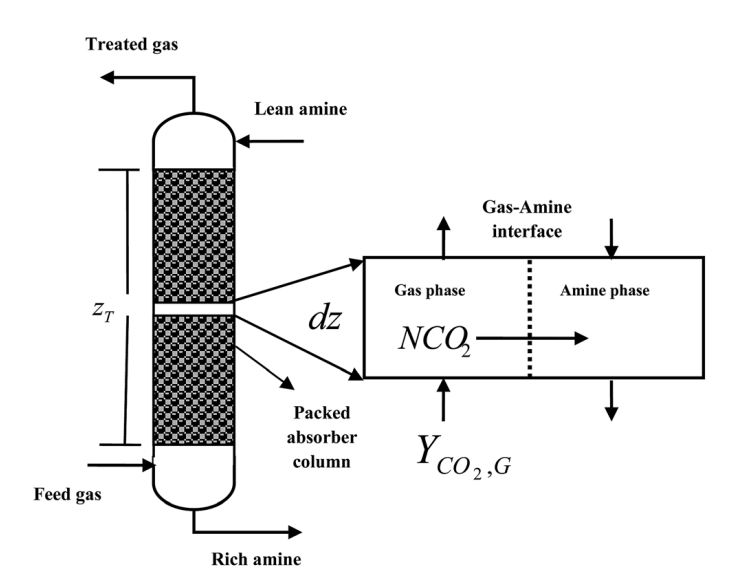
\includegraphics[width=12cm]{MEA_Absorption_Column}
                \caption{MEA Absorption Column}\label{fig:MEA Absorption Column}
            \end{figure}
            Figure~\ref{fig:MEA Absorption Column} shows a diagram of an $\mathrm{MEA}$ absorption column.
            It is a packed column with a variable height and diameter depending on the amount of liquid and vapor expected to flow into the column.
            A lean liquid solvent goes in the top and an inlet flue gas goes in the bottom.
            As the liquid descends and the vapor rises, mixing happens on the specifically designed packed element which allows both a reaction and absorption to occur, and the chosen gas species (the pollutant) is transferred from the vapor stream to the liquid stream.
            A clean outlet gas comes out at the top and a rich (saturated with the absorbed pollutant) comes out at the bottom.
            This causes a change in both mass and energy for the liquid and vapor streams as they move throughout the column.
            To simulate an absorption column, the model must track the dynamic change of the mass and energy of the liquid and vapor as it moves up or down the column.
            These dynamic changes are found as the governing equations and are in differential equation form.
            
        \subsection{Governing Equations}\label{subsec:governing-equations}
            The governing equations are the backbone of the model.
            These equations are the culmination of the absorption phenomena and entail all aspects of the thermodynamics, transport, and kinetics of the model.
            The material balances are the product of the molar flux ($N_i$) with the area at which the vapor-to-liquid transfer is happening.
            These quantities are known as interfacial area ($a_e$) and cross-sectional area ($A$).
            \begin{align}
                \frac{d \mathrm{F_{l, \mathrm{CO}_2}}}{d z} &= \mathrm{N_{\mathrm{CO}_2}} \mathrm{a}_e \mathrm{A} && \left(\frac{\unit{mol}}{\unit{s\cdot m}} \right)\\
                \frac{d \mathrm{F_{l, \mathrm{H_{2}O}}}}{d z} &=\mathrm{N_{\mathrm{H_{2}O}}} \mathrm{a}_e \mathrm{A} && \left(\frac{\unit{mol}}{\unit{s\cdot m}} \right)\\
                \frac{d \mathrm{F_{v, \mathrm{CO}_2}}}{d z} &=\mathrm{N_{\mathrm{CO}_2}} \mathrm{a}_e \mathrm{A} && \left(\frac{\unit{mol}}{\unit{s\cdot m}} \right)\\
                \frac{d \mathrm{F_{v, \mathrm{H_{2}O}}}}{d z} &=\mathrm{N_{\mathrm{H_{2}O}}} \mathrm{a}_e \mathrm{A} && \left(\frac{\unit{mol}}{\unit{s\cdot m}} \right)
            \end{align}
            We can assume that the flow rates of $\mathrm{MEA}$, $N_2$ and $O_2$ are steady-state through the column since the flux for these species across the phase boundary is negligible.
            Though flow rates are being accounted for in the differential equations, the more convenient form of mole fractions is used through the model and can be easily converted from flow rates.
            \begin{align}
                \mathrm{x}_i &= \frac{\mathrm{F}_{l, i}}{\mathrm{F}_{l, T}} \\
                \mathrm{y}_i &= \frac{\mathrm{F}_{v, i}}{\mathrm{F}_{v, T}} \\
                \mathrm{\alpha} &= \frac{\mathrm{x}_{\mathrm{CO}_2}}{\mathrm{x}_{\mathrm{MEA}}}
            \end{align}
            The energy balances are similar but instead of molar flux, it is the enthalpy flow found as ($q_l$) for the liquid and ($q_v$) for the vapor.
            The liquid flux is the sum of the heat of absorption ($q_{abs}$), heat of vaporization ($q_{vap}$), and heat transfer across the two phases ($q_{trn}$). The term in the denominator converts the enthalpy differential to a temperature differential, which is a more convenient form to work with.
            The vapor side only has heat transfer as a source or sink.
            \begin{align}
                \frac{d \mathrm{T}_l}{d z} &=\frac{\mathrm{a}_e \mathrm{A}}{\sum_i \mathrm{Cp}_i \mathrm{F}_i} \mathrm{q}_l && \left(\frac{\unit{K}}{\unit{m}} \right)\\
                \frac{d \mathrm{T}_v}{d z} &=\frac{\mathrm{a}_e \mathrm{A}}{\sum_i \mathrm{Cp}_i \mathrm{F}_i} \mathrm{q}_v && \left(\frac{\unit{K}}{\unit{m}} \right)
            \end{align}
    
            \subsubsection{Molar and Heat Flux}
                As shown above, the governing equations are mostly composed of the molar flux of each corresponding species.
                Quantifying the molar flux is paramount in accurately accounting for the amount of species being transferred from one phase to the other.
                Two parts constitute the flux equations; the driving force and the mass transfer coefficient
                \begin{align}
                    \mathrm{N}_{\mathrm{CO}_2} &= \mathrm{k}_{v, \mathrm{CO}_2}\Psi \mathrm{DF}_{\mathrm{CO}_2} && \left(\frac{\unit{mol}}{\unit{s\cdot m^2}} \right) \\
                    \mathrm{N}_{\mathrm{H_{2}O}} &= \mathrm{k}_{v, \mathrm{H_{2}O}} \mathrm{DF}_{\mathrm{H_{2}O}} && \left(\frac{\unit{mol}}{\unit{s\cdot m^2}} \right)
                \end{align}
                The driving force is governed by the thermodynamics and vapor-liquid equilibrium of the system while the mass transfer coefficients are calculated through correlations made through experimental fitting. $K_H$ is used as a correction factor for the flux of $\mathrm{CO}_2$ due to the presence of a chemical reaction in the liquid solvent.
                $\mathrm{CO}_2$ reacts with $\mathrm{MEA}$ and water to produce ions such as MEAH+ and MEACOO-.
                
                The heat flux is similar to the molar flux but has an additional enthalpy component based on the species and
                how it transfers its energy.
                The $\mathrm{CO}_2$ transfers energy via the heat of reaction/absorption due to the reaction while the water transfers energy via the heat of vaporization.
                There is also a general heat transfer between the two phases where the driving force is the temperature gradient and is contained by the overall heat transfer coefficient $\mathrm{UT}$.
                \begin{align}
                    \mathrm{q}_{abs} &= \mathrm{N}_{\mathrm{CO}_2}\mathrm{H}_{abs} && \left(\frac{\unit{J}}{\unit{s\cdot m^2}} \right)\\
                    \mathrm{q}_{vap} &= \mathrm{N}_{\mathrm{H_{2}O}}\mathrm{H}_{vap} && \left(\frac{\unit{J}}{\unit{s\cdot m^2}} \right) \\
                    \mathrm{q}_{trn} &= \mathrm{U T}\left(\mathrm{T}_v-\mathrm{T}_l\right) && \left(\frac{\unit{J}}{\unit{s\cdot m^2}} \right)\\
                    \mathrm{q}_l &= \mathrm{q}_{abs} + \mathrm{q}_{vap} + \mathrm{q}_{trn} && \left(\frac{\unit{J}}{\unit{s\cdot m^2}} \right)\\
                    \mathrm{q}_v &= \mathrm{q}_{trn} && \left(\frac{\unit{J}}{\unit{s\cdot m^2}} \right)
                \end{align}
                The formulation of both the heat of absorption and vaporization is determined through thermodynamics and the overall heat transfer coefficient is determined through transport-related correlations based on the column and packing specifications.
                
        \subsection{Thermodynamics}\label{subsec:thermodynamics}
            Of the most important concepts of the model, thermodynamics is at the core of the absorption column.
            The thermodynamics derives the driving force of the $\mathrm{CO}_2$ absorption from the vapor to the liquid.
            This driving force is the difference between the vapor and liquid fugacities.
            These fugacities can be approximated to a simpler approach depending on the complexity of the vapor-liquid-equilibrium model chosen.
            A common and rigorous approach is to use the e-NRTL activity coefficient model to determine the liquid side deviation from idealality and an equation of state for the vapor side.
            For this model, a simpler VLE model was chosen to increase the overall speed of the model.
            This simpler model has most of the deviation found in the Henry's Law formulation with parameters specifically designed to account for as many deviations as possible.
    
            \subsubsection{Driving Force}
                The following equations summarize the relevant thermodynamic relations used for the $\mathrm{CO}_2$ species.
                \begin{align}
                    \mathrm{DF}_{\mathrm{CO}_2} &= \mathrm{P}_{v, \mathrm{CO}_2} - \mathrm{P}_{l, \mathrm{CO}_2}  &&\left(\unit{Pa} \right)\\
                    \mathrm{P}_{v, \mathrm{CO}_2} &= \mathrm{P} \mathrm{y}_{\mathrm{CO}_2} && \left(\unit{Pa} \right)\\
                    P_{\mathrm{l,CO}_2} &= \exp\left(39.3 - \frac{12155}{T_{l}} - 19.0 \alpha ^2 + 1105  \frac{\alpha}{T_{l}} + 12800 \frac{\alpha ^2}{T_{l}} \right) &&\left(\unit{Pa} \right)
                \end{align}
                where $\alpha = \frac{x_{\mathrm{CO}_2}}{x_{\mathrm{MEA}}}$.
                The expression for $P_{\mathrm{l,CO}_2}$ comes from an empirical model fit by Xu and Rochelle~\cite{Xu2011TotalAmines} for a $\mathrm{MEA}$ weight fraction of .3.
                The model was regressed based on data with a temperature range of $40\,^\circ\mathrm{C} - 160\,^\circ\mathrm{C}$.
                Using this empirical model ensures very quick simulations to double-down on the purpose of this model.
                Though this brings the drawback of less potential accuracy compared to a more rigorous model the e-NRTL activity coefficient model or ePC-SAFT equation of state model.
                With less rigor though brings much more stability and consistency which is important when attempting to run a model for many simulations
                The following equations used for water are
                \begin{align}
                    \mathrm{DF}_{\mathrm{H_{2}O}} &= \mathrm{P}_{v, \mathrm{H_{2}O}} - \mathrm{P}_{l, \mathrm{H_{2}O}} && \left(\unit{Pa} \right)\\
                    \mathrm{P}_{v, \mathrm{H_{2}O}} &= \mathrm{P} \mathrm{y}_{\mathrm{H_{2}O}} && \left(\unit{Pa} \right)\\
                    \mathrm{P}_{l, \mathrm{H_{2}O}} &= \mathrm{P}_{sat, \mathrm{H_{2}O}} \mathrm{x}_{\mathrm{H_{2}O}} && \left(\unit{Pa} \right)
                \end{align}
            
            \subsubsection{Henry's Law}
                To formulate a Henry's Law for the mixture of the liquid solvent, the N2O analogy is used.
                Below are the equations that help reach the expressions for the solubility of $\mathrm{CO}_2$ in $\mathrm{MEA}$(Jiru)
                \begin{align}
                    H_{\mathrm{N_{2}O},\mathrm{MEA}} &= \left(2.448 \times 10^5\right) e^{-1348/T_l} && \left(\frac{\unit{Pa} \cdot \unit{m}^3}{\unit{mol}} \right)\\
                    H_{\mathrm{CO}_2, \mathrm{H_{2}O}} &= \left(3.52 \times 10^6\right) e^{-2113/T_l} && \left(\frac{\unit{Pa} \cdot \unit{m}^3}{\unit{mol}} \right)\\
                    H_{\mathrm{N_{2}O},\mathrm{H_{2}O}} &= \left(8.449 \times 10^6\right) e^{-2283/T_l} && \left(\frac{\unit{Pa} \cdot \unit{m}^3}{\unit{mol}} \right)\\
                    H_{\mathrm{CO}_2,\mathrm{MEA}} &= H_{\mathrm{N_{2}O},\mathrm{MEA}} \frac{H_{\mathrm{CO}_2, \mathrm{H_{2}O}}}{H_{\mathrm{N_{2}O},\mathrm{H_{2}O}}} && \left(\frac{\unit{Pa} \cdot \unit{m}^3}{\unit{mol}} \right)
                \end{align}
                Next, the deviation is formulated since the solution is not ideal due to the intermolecular forces between the $\mathrm{MEA}$, $\mathrm{CO}_2$, and water.
                The $Ra$ term is used as the deviation from ideal solubility and uses terms $a_1$, $a_2$, $a_3$, and $b$ coefficients in the functional form.
                This formulation was created from (Reference).
                \begin{align}
                    Ra_1 &= \left(a_1+a_2 \left(T_l-273.15\right)+a_3 \left(T_l-273.15\right)^2+b w_{\mathrm{H_{2}O}} \right) \\
                    Ra_2 &= Ra_1 w_{\mathrm{MEA}} w_{\mathrm{H_{2}O}} \\
                    \sigma &= w_{\mathrm{MEA}} \ln\left(H_{\mathrm{CO}_2,\mathrm{MEA}}\right)+w_{\mathrm{H_{2}O}} \ln\left(H_{\mathrm{CO}_2,\mathrm{H_{2}O}}\right) \\
                    H_{\mathrm{CO}_2,mix} &= e^{Ra + \sigma} && \left(\frac{\unit{Pa} \cdot \unit{m}^3}{\unit{mol}} \right)
                \end{align}
            
            \subsubsection{Enthalpy}
                The enthalpy of the system plays a big role in the energy balance of the system.
                Due to the substantial swing of water from one phase to the other, the heat of vaporization will determine the location of the temperature bulge combined with the heat of absorption.
                Fortunately, there are reasonable assumptions that can be made for both values with high accuracy.
                \begin{align}
                    H_{abs} &= -82000 && \left(\frac{\unit{J}}{\unit{mole}} \right) \\
                    H_{vap} &= -48000 && \left(\frac{\unit{J}}{\unit{mole}} \right)
                \end{align}
                The main concern with the enthalpy flow arises when it's combined with the molar flux of either $\mathrm{CO}_2$ or $H_{2}O$.
                Both the magnitude and the direction of the molar flux will greatly influence the enthalpy flux and thus the temperature swing of the column.
                While thermodynamics corresponds to the driving force, transport correlations are needed to compute the mass transfer coefficients.
    
        \subsection{Transport}\label{subsec:transport}
            
            The transport properties govern the flow of overall substance within the column.
            Of the properties, the mass transfer coefficients are terms that quantify the resistance of transfer that each species has between the proposed barrier.
            This resistance is quantified with the dimensions of the column, the type and size of the packing, and the properties of the liquid and vapor mixtures.
            Each of the relevant properties is found using the temperature and composition as inputs and a functional correlation with tuned parameters.
            The relevant properties used are density, viscosity, diffusivity, and surface tension.
            These properties will be covered later in the paper.
            Within transport, you can differentiate between the two types of transfer, mass-transfer and heat-transfer.
            Evaluating the mass-transfer component of the absorption simulation is critical in obtaining and accurate flux of $\mathrm{CO}_2$ that is being absorbed.
            The heat-transfer component plays a role in the energy balance between the two phases present in the column
    
            `\subsubsection{Inter-facial Area and Liquid Holdup}
            
                Two mass-transfer properties of relevance found in absorber simulations are interfacial area and liquid holdup.
                The interfacial area is the area in which the transfer happens and is dependent on the density, surface tension, and a packing constant.
                It is found both in the final molar flux equation as well a part of the mass transfer coefficients.
                The liquid holdup is the volume of liquid held per volume of a packed bed under operating conditions.
                It is found in each of the mass transfer coefficient equations given by Chinen and Tsai~\cite{SoaresChinen2018DevelopmentQuantification,Tsai2010MassPacking}
                \begin{align}
                    a_e &=1.42 a_p\left[\frac{\rho_L}{\sigma_L} g^{1 / 3}\left(\frac{u_L}{a_p}\right)^{4 / 3}\right]^{0.116} && \left(\frac{\unit{m}^2}{\unit{m}^3} \right) \\
                    h_L &= 11.45\left[\frac{u_L}{S^2 g^{2 / 3} a_p}\left(\frac{\mu_L}{\rho_L}\right)^{1 / 3}\right]^{0.6471} && \left(\unit{m}^3 \right)\\
                    h_V &= \epsilon - h_L && \left(\unit{m}^3 \right)
                \end{align}

            \subsubsection{Mass Transfer Coefficients}
            
                The mass transfer coefficients for vapor and liquid depend on several components such as densities, viscosities, surface tension, flow velocities, specific surface area, void fraction, and other packing-specific constants.
                These constants are found through regression with a large database for multiple types of packing and sizes by Billet and Chinen\cite{Billet1999PredictionPackings, SoaresChinen2018DevelopmentQuantification}.
                \begin{align}
                    k_l &= C_L \cdot 12^{1 / 6}\left(\frac{u_L}{h_L}\right)^{1 / 2}\left(\frac{D_L}{d_h}\right)^{1 / 2} && \left(\frac{\unit{m} }{\unit{s}} \right)\\
                    k_v &=\frac{C_{\mathrm{V}}D_{\mathrm{V}}}{RT_v} \left(\frac{a_p}{d_h h_V}\right)^{1/2}  \left(\frac{u_{\mathrm{v}} \rho_{\mathrm{V}}}{a_p \mu_{\mathrm{V}}}\right)^{3 / 4}\left(\frac{\mu_{\mathrm{V}}}{\rho_{\mathrm{V}} D_{\mathrm{V}}}\right)^{1 / 3} && \left(\frac{\unit{mol} }{\unit{Pa} \cdot{m}^2 \cdot \unit{s}} \right)
                \end{align}
            
            \subsubsection{Enhancement Factor}
            
                The enhancement factor is defined as the ratio of mass transfer from chemical absorption compared to physical absorption.
                It is therefore a relative factor which indicates the improvements of a reactive solvent compared to a physical non-reactive solvent.
                The enhancement factor is preferred in process simulations since it reduces the computational load.
                The chosen model to compute the enhancement factor comes from Gaspar\cite{Gaspar2015ACase-study} which is solved by solving a system of two non-linear equations.
                The following equations can be defined outside the non-linear system of equations
                \begin{align}
                    k_2 &= 3.1732 \times 10^{9} \exp\left( \frac{-4936.6}{T_l}\right) \\
                    Ha &= \frac{\sqrt{k_2 C_{l,\mathrm{MEA},true} D_{l,\mathrm{CO}_2}}}{k_{l,\mathrm{CO}_2}} \\
                \end{align}
                $k_2$ is the rate of the chemical reaction that governs the consumption of $\mathrm{MEA}$
                $\mathrm{Ha}$ is the Hatta number which compares the rate of reaction in a liquid film to the rate of diffusion through the film.
                The following equations are intermediate expressions contained within the system of equations that are solved that are dependent on $\mathrm{E}$ and $\Upsilon _{\mathrm{CO}_2}.$
                \begin{align}
                    \Psi &= \frac{E \frac{k_{l, \mathrm{CO}_2}}{k_{v, \mathrm{CO}_2}}}{E \frac{k_{l, \mathrm{CO}_2}}{k_{v, \mathrm{CO}_2}} + H_{\mathrm{CO}_2, mix}} \\
                    \mathrm{C}_{l, \mathrm{CO}_2}^{*} &= \frac{\frac{y_{\mathrm{CO}_2}P}{\Psi} + C_{l, \mathrm{CO}_2, true}}{\frac{H_{\mathrm{CO}_2,mix}}{\Psi} + 1}
                \end{align}
                $\Psi$ represents the overall correction factor for the driving force of $\mathrm{CO_2}$ due to the Henry's Law and the present reactions.
                $\mathrm{C}_{l, \mathrm{CO}_2}^{*}$ is the liquid concentration of $\mathrm{CO_2}$ at the interface.
                \begin{align}
                    \Upsilon_{\mathrm{CO}_2}^b &= \frac{C_{l, \mathrm{CO}_2, true}}{C_{l, \mathrm{CO}_2}^*} \\
                    \Upsilon_{\mathrm{MEAH}^{+}} &= 1+\frac{D_{l, \mathrm{MEAH}^{+}} C_{l,\mathrm{MEA}, true}}{2 D_{l, \mathrm{MEAH}^{+}} C_{l, \mathrm{MEAH}^{+}, true}}\left(1-\Upsilon_{\mathrm{MEA}}\right) \\
                    \Upsilon_{\mathrm{MEACOO}^{-}} &= 1+\frac{D_{l, \mathrm{MEACOO}^{-}} C_{l,\mathrm{MEA}, true}}{2 D_{l, \mathrm{MEACOO}^{-}} C_{l, \mathrm{MEACOO}^{-}, true}}\left(1-\Upsilon_{\mathrm{MEA}}\right) \\
                    \Upsilon_{\mathrm{CO}_2}^* &= \Upsilon_{\mathrm{CO}_2}^b \Upsilon_{\mathrm{MEAH}^{+}} \Upsilon_{\mathrm{MEACO}^-}\left(\Upsilon_{\mathrm{MEA}}\right)^{-2}
                \end{align}
                These equations represent dimensionless concentration quantities for each relevant species at bulk or interface
                \begin{align}
                    E_{\infty}^* &= 1+\frac{D_{l,\mathrm{MEA}} C_{l, \mathrm{MEA}}^{\mathrm{t}}}{2 D_{l, \mathrm{CO}_2} C_{l, \mathrm{CO}_2}^*}
                \end{align}
                While $E_{\infty}^*$ is the instantaneous enhancement factor.
                The following equations constitute the governing equations for the two equations two unknowns system.
                \begin{align}
                    E &= 1+\left(E_{\infty}^*-1\right) \frac{\left(1-\Upsilon_{\mathrm{MEA}}\right)}{\left(1-\Upsilon_{\mathrm{CO}_2}^b\right)} \\
                    E &= Ha \sqrt{\Upsilon_{\mathrm{MEA}}} \frac{1-\mathrm{\Upsilon}_{\mathrm{CO}_2}^*}{1-\mathrm{\Upsilon}_{\mathrm{CO}_2}^b}
                \end{align}
                A simple root solving method can obtain $\mathrm{E}$ and can then obtain $\Psi$ to use in correcting the driving force of $\mathrm{CO_2}$
            
        \subsubsection{Heat-Transfer}
        
    
        \subsection{Properties}\label{subsec:properties}
                
                \subsubsection{Liquid Properties}
        
                    Density
                    \begin{align}
                        V_{\mathrm{MEA}} &=  \frac{MW_{\mathrm{MEA}}}{a_1 T_l^2 + b_1 T_l + c_1} \\
                        V_{\mathrm{H_{2}O}} &=  \frac{MW_{\mathrm{H_{2}O}}}{a_2 T_l^2 + b_2 T_l + c_2} \\
                        V_{\mathrm{CO}_2} &=  a + (b + c x_{\mathrm{MEA}}) x_{\mathrm{MEA}} x_{\mathrm{H_{2}O}} + (d + e x_{\mathrm{MEA}}) x_{\mathrm{MEA}} x_{\mathrm{CO}_2} \\
                        V_l &= V_{\mathrm{CO}_2}x_{\mathrm{CO}_2} + V_{\mathrm{MEA}}x_{\mathrm{MEA}} + V_{\mathrm{H_{2}O}}x_{\mathrm{H_{2}O}} \\
                        \rho _{l,mol} &= \frac{1}{V_l} \\
                        \rho _{l,mass} &= \rho _{l,mol}MW_{T,l}
                    \end{align}
        
                    Diffusivity
                    \begin{align}
                        D_{l, \mathrm{CO}_2} = (a + b C_{\mathrm{MEA}} + c C_{\mathrm{MEA}}^2) e^{\frac{d + e C_{\mathrm{MEA}}}{T_l}}
                    \end{align}
        
                    Viscosity
                    
                    \begin{align}
                        \mu _{l,\mathrm{H_{2}O}} &= 1.002 \times 10^(\frac{1.3272(293.15 - T_l - c(T_l - 293.15)^2)}{T_l - 168.15} \\
                        \mu _{l,mix} &= \mu _{l,\mathrm{H_{2}O}} \times e^{\frac{\left(\left(a r+b\right) T_l+c W_{\mathrm{MEA}}+d\right) \left(\alpha \left(e r+f T_l+g\right)+1\right) r}{{T_l}^2}}
                    \end{align}
        
                    Surface Tension
                    
                    \begin{align}
                        \sigma _{\mathrm{CO}_2} &= S_1 r^2+S_2 r+S_3+T_l \left(S_4 r^2+S_5 r+S_6\right) \\
                        \sigma _{\mathrm{MEA}} &= c_{1,\mathrm{MEA}} \left(1-\frac{T_l}{T_{c,\mathrm{MEA}}}\right)^{c_{2,\mathrm{MEA}}+c_{3,\mathrm{MEA}} \frac{T_l}{T_{c,\mathrm{MEA}}}+c_{4,\mathrm{MEA}} \left(\frac{Tl}{T_{c,\mathrm{MEA}}}\right)^2} \\
                        \sigma _{\mathrm{H_{2}O}} &= c_{1,\mathrm{H_{2}O}} \left(1-\frac{T_l}{T_{c,\mathrm{H_{2}O}}}\right)^{c_{2,\mathrm{H_{2}O}}+c_{3,\mathrm{H_{2}O}} \frac{T_l}{T_{c,\mathrm{H_{2}O}}}+c_{4,\mathrm{H_{2}O}} \left(\frac{Tl}{T_{c,\mathrm{H_{2}O}}}\right)^2} \\
                        A &= a+b \alpha+c {\alpha}^2+d w_{\mathrm{MEA}}+e {w_{\mathrm{MEA}}}^2 \\
                        B &= f+g \alpha+h {\alpha}^2+i w_{\mathrm{MEA}}+j {w_{\mathrm{MEA}}}^2 \\
                        \sigma _{mix} &= \sigma_{\mathrm{H_{2}O}}+\left(\sigma_{\mathrm{CO}_2}-\sigma_{\mathrm{H_{2}O}}\right) A x_{\mathrm{CO}_2}+\left(\sigma_{\mathrm{MEA}}-\sigma_{\mathrm{H_{2}O}}\right) B x_{\mathrm{MEA}}
                    \end{align}
                
        
            \subsubsection{Vapor Properties}
                Density
                \begin{align}
                    \rho _{v,mol} &= \frac{P}{RT_v} \\
                    \rho _{v,mass} &= \rho _{v,mol} \times MW_{v,T}
                \end{align}
                
                Viscosity
                \begin{align}
                    \mu _{v,\mathrm{CO}_2} &= \frac{2.148 \times 10^{-6} \ T_v^{0.46}}{1+\frac{290}{T_v}} \\
                    \mu _{v,\mathrm{H_{2}O}} &= 1.7096\times 10^{-8} \ T_v^{1.1146} \\
                    \mu _{v,N_2} &= \frac{6.5592\times 10^{-7} \ T_v^{0.6081}}{1+\frac{54.714}{T_v}} \\
                    \mu _{v,O_2} &= \frac{5.5462\times 10^{-8} \ T_v^{0.8825}}{1+\frac{73.316}{T_v}} \\
                    \mu _{v,mix} &= e^{\ln\left(mu_{v,\mathrm{CO}_2}\right) y_{\mathrm{CO}_2}+\ln\left(mu_{v,\mathrm{H_{2}O}}\right) y_{\mathrm{H_{2}O}}+\ln\left(mu_{v,N_2}\right) y_{N_2}+\ln\left(mu_{v,O_2}\right) y_{O_2}}
                \end{align}
                
                Diffusivity
                \begin{align}
                    D _{v,\mathrm{CO}_2} &= 8.7 \times 10^{-5} \ T_v^{1.75} \\
                    D _{v,\mathrm{H_{2}O}} &= 1.2 \times 10^{-4} \ T_v^{1.75} \\
                    D _{v,N_2} &= 9.5 \times 10^{-5} \ T_v^{1.75} \\
                    D _{v,O_2} &= 1.16\times 10^{-4} \ T_v^{1.75}
                \end{align}
        
        \subsubsection{Intermediates}
        
            An important component of modeling is using convenient state variables to manage the model and most often those are found as liquid ($x_i$) and vapor ($y_i$) mole fractions and liquid ($C_{l,i}$) and vapor ($C_{v,i}$) concentrations since they are compatible with most sub-models found rather than flowrate.
            The concentrations are just abbreviations from the density of each stream which is found using a function correlation model discussed below.
            Those are defined as such below.
            Another important variable is the lean loading ($\alpha$) which symbolizes the amount of initial $\mathrm{CO}_2$ present in the lean solution before absorption occurs.
            This value is important since almost all factors in the model are dependent on this value.
        
            \begin{align}
                \mathrm{x}_i &= \frac{\mathrm{F}_{l, i}}{\mathrm{F}_{l, T}} \\
                \mathrm{y}_i &= \frac{\mathrm{F}_{v, i}}{\mathrm{F}_{v, T}} \\
                \mathrm{\alpha} &= \frac{\mathrm{x}_{\mathrm{CO}_2}}{\mathrm{x}_{MEA}} \\
                \mathrm{C}_{l, i} &= \mathrm{x}_i \mathrm{\rho}_{l, mol} \\
                \mathrm{C}_{v, i} &= \mathrm{y}_i \mathrm{\rho}_{v, mol} \\
                u_l &= \frac{\mathrm{F}_{l,T}}{\mathrm{A} \rho _{l,mol}} \\
                u_v &= \frac{\mathrm{F}_{v,T}}{\mathrm{A} \rho _{v,mol}}
            \end{align}
            
    \section{Simulating}\label{sec:simulating}
        
        \subsection{Integrating}\label{subsec:integrating}
        
        \subsection{Shooting}\label{subsec:shooting}
        
    \section{Discussion}\label{sec:discussion}
        
        \subsection{Results}\label{subsec:results}
        
        \subsection{Analysis}\label{subsec:analysis}
        
    \section{Limitations}\label{sec:limitations}
        
        \subsection{Regime}\label{subsec:regime}
        
        \subsection{Convergence}\label{subsec:convergence}
    
    \section{Conclusion}\label{sec:conclusion}
        
        \newpage
    
    \printbibliography

\end{document}
